\documentclass[a4paper,12pt]{article}

\usepackage[utf8]{inputenc}
\usepackage[left=0.5in,right=0.5in,top=1in,bottom=1in]{geometry}
\usepackage{amsmath,amssymb,amsfonts,mathtools}
\usepackage{pgfplots,graphicx,calc,changepage}
\pgfplotsset{compat=newest}
\usepackage{enumitem}
\usepackage{fancyhdr}
\usepackage[colorlinks = true, linkcolor = blue]{hyperref}

\newcommand{\nats}{\mathbb{N}}
\newcommand{\reals}{\mathbb{R}}
\newcommand{\rats}{\mathbb{Q}}
\newcommand{\ints}{\mathbb{Z}}
\newcommand{\pols}{\mathcal{P}}
\newcommand{\cants}{\Delta\!\!\!\!\Delta}
\newcommand{\eps}{\varepsilon}
\newcommand{\st}{\backepsilon}
\newcommand{\abs}[1]{\left| #1 \right|}
\newcommand{\dom}[1]{\mathrm{dom}\left(#1\right)}
\newcommand{\erf}{\mathrm{erf}}
\newcommand{\for}{\text{ for }}
\newcommand{\dd}[1]{\mathrm{d}#1}
\newcommand{\spn}{\mathrm{sp}}
\newcommand{\nul}{\mathcal{N}}
\newcommand{\col}{\mathrm{col}}
\newcommand{\rank}{\mathrm{rank}}
\newcommand{\norm}[1]{\lVert #1 \rVert}
\newcommand{\inner}[1]{\left\langle #1 \right\rangle}
\newcommand{\pmat}[1]{\begin{pmatrix} #1 \end{pmatrix}}
\renewcommand{\and}{\text{ and }}

\newsavebox{\qed}
\newenvironment{proof}[2][$\square$]
    {\setlength{\parskip}{0pt}\par\textit{Proof:} #2\setlength{\parskip}{0.25cm}
        \savebox{\qed}{#1}
        \begin{adjustwidth}{\widthof{Proof:}}{}
    }
    {
        \hfill\usebox{\qed}\end{adjustwidth}
    }

\pagestyle{fancy}
\fancyhead{}
\lhead{Caleb Jacobs}
\chead{APPM 5470: PDEs}
\rhead{Homework \#3}
\cfoot{}
\setlength{\headheight}{35pt}
\setlength{\parskip}{0.25cm}
\setlength{\parindent}{0pt}

\begin{document}
\section*{Book Problems}
\begin{enumerate}[label = \arabic*.]
    \item Chapter 4, Problem 10: Let $ f(x,t) $ be a continuous function, and let $ \Delta(x,t) $ denote the domain of dependence of the point $ (x,t) $ for 
    \[
    	u_{tt} = c^2 u_{xx}.
    \]
    Show that $ u(x,t) = \frac{1}{2c} \iint_{\Delta(y, \tau)} f(x,t)\dd y \dd \tau $ satisfies
    \[
    	u_{tt} = c^2 u_{xx} + f(x,t), u(x,0) = 0 = u_t(x,0).
    \]
    
    First, let's rewrite $ u $ with more solid bounds:
    \[
    	u(x,t) = \frac{1}{2c} \int_0^t \int_{c (\tau - t) + x}^{-c(\tau - t) + x} f(y,\tau) \dd y \dd \tau.
    \]
    Then, using Leibniz integral rule, our  derivatives become
    \begin{align*}
    	u_{tt} &= \frac{1}{2c} \frac{\partial}{\partial t} \left(c \int_{0}^{t} f(c(t - \tau) + x, \tau) + f(-c(t - \tau) + x) \dd \tau \right) \\
    	&=  f(x,t) + \frac{1}{2c}c^2 \int_{0}^{t} f_x(c(t - \tau) + x, \tau) - f_x(-c(t - \tau) + x) \dd \tau \\
    	u_{xx} &= \frac{1}{2c} \frac{\partial}{\partial x} \left(\int_{0}^{t} f(c(t - \tau) + x, \tau) - f(-c(t - \tau) + x) \dd \tau \right) \\
    	&= \frac{1}{2c} \int_{0}^{t} f_x(c(t - \tau) + x, \tau) - f_x(-c(t - \tau) + x) \dd \tau.
    \end{align*}
	Then, our PDE becomes
	\begin{align*}
		u_{tt} - c^2 u_{xx}  - f(x,t) &= f(x,t) + \frac{1}{2c}c^2 \int_{0}^{t} f_x(c(t - \tau) + x, \tau) - f_x(-c(t - \tau) + x) \dd \tau \\
		&- c^2 \frac{1}{2c} \int_{0}^{t} f_x(c(t - \tau) + x, \tau) - f_x(-c(t - \tau) + x) \dd \tau - f(x,t) \\
		&= f(x,t) + \frac{c}{2} \int_{0}^{t} f_x(c(t - \tau) + x, \tau) - f_x(-c(t - \tau) + x) \dd \tau \\
		&- \frac{c}{2} \int_{0}^{t} f_x(c(t - \tau) + x, \tau) - f_x(-c(t - \tau) + x) \dd \tau - f(x,t) \\
		&= 0.
	\end{align*}
	So $ u $ satisfies the PDE, now let's check the initial conditions
	\begin{align*}
		u(x,0) &= \frac{1}{2c} \int_0^0 \int_{c (\tau - 0) + x}^{-c(\tau - 0) + x} f(y,\tau) \dd y \dd \tau = 0 \\
		u_t(x,0) &= \frac{1}{2} \int_{0}^{0} f(c(0 - \tau) + x, \tau) + f(-c(0 - \tau) + x) \dd \tau = 0.
	\end{align*}
	Thus, $ u $ solves the IVP.
     
    \item Chapter 5, Problem 6: Solve the heat equation with initial condition $ u(x,0) = H(x)e^{-x} $ where
    \[
    	H(x) = \begin{cases}
    		0, & x < 0 \\
    		1, & 0 \leq x
    	\end{cases}.
    \]
    
    Using the fundamental solution, we have
    \begin{align*}
    	u(x,t) &= \frac{1}{\sqrt{4 \pi k t}} \int_{-\infty}^{\infty}e^{-\frac{(x - y)^2}{4 k t}} H(y)e^{-y} \dd y \\
    	&= \frac{1}{\sqrt{4 \pi k t}} \int_{0}^{\infty}e^{-\frac{(x - y)^2}{4 k t}}e^{-y} \dd y \\
    	&= -\frac{1}{\sqrt{4 \pi k t}} \int_{x}^{-\infty}e^{-\frac{u^2}{4 k t}}e^{u - x} \dd u \\
    	&= -\frac{1}{\sqrt{4 \pi k t}} \int_{x}^{-\infty}e^{-\frac{1}{4 k t}(u^2 - 4ktu)}e^{- x} \dd u \\
    	&= -\frac{1}{\sqrt{4 \pi k t}} \int_{x}^{-\infty}e^{-\frac{1}{4 k t}(u^2 - 4ktu + (2kt)^2 - (2kt)^2)}e^{- x} \dd u \\
    	&= -\frac{1}{\sqrt{4 \pi k t}} \int_{x}^{-\infty}e^{-\frac{1}{4 k t}(u - 2kt)^2}e^{kt - x} \dd u \\
    	&= e^{kt - x}\frac{1}{\sqrt{4 \pi k t}} \int_{-\infty}^{x}e^{-\left(\frac{u}{2\sqrt{kt}} - \sqrt{kt}\right)^2} \dd u \\
    	&= e^{kt - x}\frac{2 \sqrt{k t}}{\sqrt{4 \pi k t}} \int_{-\infty}^{\frac{x}{2\sqrt{kt}} - \sqrt{kt}}e^{-v^2} \dd v \\
    	&= e^{kt - x}\frac{1}{\sqrt{\pi}} \int_{-\infty}^{\frac{x}{2\sqrt{kt}} - \sqrt{kt}}e^{-v^2} \dd v \\
    	&= e^{kt - x}\frac{1}{\sqrt{\pi}} \frac{\sqrt{\pi}}{2} \left(1 + \erf\left(\frac{x}{2\sqrt{kt}} - \sqrt{kt}\right)\right) \\
    	&= \frac{1}{2} e^{kt - x} \left(1 + \erf\left(\frac{x}{2\sqrt{kt}} - \sqrt{kt}\right)\right).
    \end{align*}
\end{enumerate}

\section*{Additional Problems}
\begin{enumerate}[label = \arabic*.]
	\item The integral form of Maxwell's equation can be written:
	\begin{align}
		\text{Gauss' law:}&\quad \int_{\partial \Omega} \textbf{D}\cdot \textbf{n} \dd S = 0 \label{equ:gauss} \\
		\text{no magnetic charge:}&\quad \int_{\partial\Omega} \textbf{B} \cdot \textbf{n} \dd S = 0 \label{equ:charge} \\
		\text{Amp\`ere's law:}&\quad \int_{\partial \Sigma} \textbf{H} \cdot \textbf{n} \dd l - \frac{\dd}{\dd t} \int_\Sigma \textbf{D} \cdot \textbf{n} \dd S = 0 \label{equ:amps} \\
		\text{Faraday's law:}&\quad \int_{\partial \Sigma} \textbf{E} \cdot \textbf{n} \dd l - \frac{\dd}{\dd t} \int_\Sigma \textbf{B} \cdot \textbf{n} \dd S = 0 \label{equ:faraday}
	\end{align}
	where $ \Omega \subset \reals^3 $ is any three-dimensional volume and $ \partial \Omega $ is its boundary, $ \Sigma \subset \reals^3 $ is any two-dimensional surface and $ \partial \Sigma $ is its boundary, and $ \textbf{D}, \textbf{B}, \textbf{H}, \textbf{E} $ are smooth vector fields mapping $ \reals^3 \times \reals $ to $ \reals^3 $.
	\begin{enumerate}[label = (\alph*)]
		\item Express Maxwell's equation in local, differential form.
		
		Using the divergence theorem and Stoke's theorem, we have
		\begin{align*}
			\eqref{equ:gauss} & \int_{\partial \Omega} \textbf{D}\cdot \textbf{n} \dd S = \int_\Omega \nabla \cdot \textbf{D} \dd V = 0 \implies \nabla \cdot \textbf{D} = 0 \\
			\eqref{equ:charge} & \int_{\partial\Omega} \textbf{B} \cdot \textbf{n} \dd S = \int_\Omega \nabla \cdot \textbf{B} \dd V = 0 \implies \nabla \cdot \textbf{B} = 0 \\
			\eqref{equ:amps} & \int_{\partial \Sigma} \textbf{H} \cdot \textbf{n} \dd l - \frac{\dd}{\dd t} \int_\Sigma \textbf{D} \cdot \textbf{n} \dd S = \int_\Sigma (\nabla \times \textbf{H}) \cdot \textbf{n} \dd S - \int_\Sigma \frac{\dd}{\dd t} \textbf{D} \cdot \textbf{n} \dd S \\
			&= \int_\Sigma (\nabla \times \textbf{H}) \cdot \textbf{n} - \frac{\dd}{\dd t} \textbf{D} \cdot \textbf{n} \dd S = 0 \implies \nabla \times \textbf{H} = \frac{\dd \textbf{D}}{\dd t}\\
			\eqref{equ:faraday} & \int_{\partial \Sigma} \textbf{E} \cdot \textbf{n} \dd l - \frac{\dd}{\dd t} \int_\Sigma \textbf{B} \cdot \textbf{n} \dd S = \int_\Sigma (\nabla \times \textbf{E}) \cdot \textbf{n} \dd S - \int_\Sigma \frac{\dd}{\dd t} \textbf{B} \cdot \textbf{n} \dd S \\
			&= \int_\Sigma (\nabla \times \textbf{E}) \cdot \textbf{n} - \frac{\dd}{\dd t} \textbf{B} \cdot \textbf{n} \dd S = 0 \implies \nabla \times \textbf{E} = \frac{\dd \textbf{B}}{\dd t}\\
		\end{align*}
		
		\item Assuming the constitutive laws
		\[
			\textbf{D} = \epsilon \textbf{E}, \quad \textbf{B} = \mu \textbf{H}
		\]
		where $ \varepsilon > 0 $ and $ \mu > 0 $, derive the $ (3 + 1)D $ (Vector) linear wave equation for the electric field $ \textbf{E} $ and the magnetic field \textbf{H}. What is the electromagnetic wave speed?
		
		Using the constitutive laws, we can rewrite Maxwell's local differential equations as
		\begin{align}
			\varepsilon \nabla \cdot \textbf{E} &= 0 \label{equ:E} \\
			\mu \nabla \cdot \textbf{H} &= 0 \label{equ:H} \\
			\nabla \times \textbf{H} &= \varepsilon \textbf{E}_t\label{equ:nablaH}\\
			\nabla \times \textbf{E} &= -\mu \textbf{H}_t \label{equ:nablaE}.
		\end{align}
		Now, we can start deriving the electromagnetic linear wave equations. From \eqref{equ:nablaH}, we have
		\begin{align*}
			\frac{\partial}{\partial t} \nabla \times \textbf{H} = \varepsilon \frac{\partial}{\partial t} \textbf{E}_t &\implies \nabla \times \textbf{H}_{t} = \varepsilon\textbf{E}_{tt} \\
			\text{which from \eqref{equ:nablaE}} &\implies -\frac{1}{\mu} \nabla \times \nabla \times \textbf{E} = \varepsilon \textbf{E}_{tt} \\
			&\implies -\frac{1}{\mu}(\nabla (\nabla \cdot \textbf{E}) - \nabla^2 \textbf{E}) = \varepsilon \textbf{E}_{tt} \\
			&\implies \varepsilon \textbf{E}_{tt} - \frac{1}{\mu} \nabla^2 \textbf{E} = -\frac{1}{\mu} \nabla (\nabla \cdot \textbf{E}) \\
			\text{which by \eqref{equ:E}} &\implies \textbf{E}_{tt} - \frac{1}{\mu \varepsilon} \nabla^2 \textbf{E} = \textbf{0}
		\end{align*}
		Now, by the same process, we can get the other wave equation. From \eqref{equ:nablaH}
		\begin{align*}
			\frac{\partial}{\partial t} \nabla \times \textbf{E} = -\mu \textbf{H}_{tt} &\implies \nabla \times \textbf{E}_t = -\mu \textbf{H}_{tt} \\
			\text{which by \eqref{equ:nablaE}} &\implies \frac{1}{\varepsilon} \nabla \times \nabla \times \textbf{H} = -\mu \textbf{H}_{tt} \\
			&\implies \frac{1}{\varepsilon}(\nabla (\nabla \cdot \textbf{H}) - \nabla^2\textbf{H}) = -\mu \textbf{H}_{tt}\\
			&\implies \mu \textbf{H}_{tt} - \frac{1}{\varepsilon} \nabla^2 \textbf{H} = \frac{1}{\varepsilon}\nabla (\nabla \cdot \textbf{H}) \\
			\text{which by \eqref{equ:H}} &\implies \textbf{H}_{tt} - \frac{1}{\mu \varepsilon} \nabla^2 \textbf{H} = \textbf{0}.
		\end{align*}
		Thus, our electromagnetic wave equations are given by 
		\begin{align*}
			\textbf{E}_{tt} - \frac{1}{\mu \varepsilon} \nabla^2 \textbf{E} &= \textbf{0} \\
			\textbf{H}_{tt} - \frac{1}{\mu \varepsilon} \nabla^2 \textbf{H} &= \textbf{0}
		\end{align*}
		where the wave speed is given by $ \sqrt{\frac{1}{\mu \varepsilon}} $. On a fun note, in a vacuum, this wave speed actually becomes the speed of light and so we can see that electromagnetic waves travel at the speed of light!
	\end{enumerate}	
	
	\item Assuming the following initial value problems have a solution, determine whether or not that solution is unique, justifying your answer. Assume $ u $ is twice continuously differentiable and its first and second derivatives are $ L^2 $ integrable.
	
	\textit{Note, because our functions are $ L^2 $ integrable up to the second derivative, boundary evaluations at $ \pm\infty $ must go to zero.}
	\begin{enumerate}[label = (\alph*)]
		\item Inhomogeneous wave equation with boundary:
		\[	
			\begin{cases}
				u_{tt} - c^2 u_{xx} + f(x,t), & c > 0, x > 0, t > 0 \\
				u(x,0) = \phi(x), u_t(x,0) = \psi(x), & x > 0 \\
				u(0, t) = h(t), & t > 0.
			\end{cases}
		\]
		
		To check the uniqueness of this problem, suppose we have to solutions to the IVBP, $ u_1 $ and $ u_2 $. Then by linearity, $ v(x,t) = u_1 - u_2 $ is a solution to the IVBP
		\[
			\begin{cases}
				v_{tt} - c^2 v_{xx} = 0, & c > 0, x > 0, t > 0 \\
				v(x, 0) = 0, v_t(x,0) = 0, & x > 0 \\
				u(0,t) = 0, & t > 0
			\end{cases}.
		\]
		From the boundary condition we must have
		\[
			u_t(0, t) = 0.
		\]
		Now, consider $ v_t (v_{tt} - c^2 v_{xx}) = 0 $. Integrating yields
		\begin{align*}
			& \int_0^\infty v_t v_{tt} \dd x - c^2 \int_0^\infty v_t v_{xx} \dd x = 0 \\
			\implies & \int_{0}^{\infty} \partial_t \left(\frac{1}{2} v_t^2\right) \dd x - \left.c^2 v_t v_x \right|_{x=0}^\infty + c^2 \int_{0}^{\infty}v_x v_{xt} \dd x = 0 \\
			\implies & \int_{0}^{\infty} \partial_t \left(\frac{1}{2} v_t^2\right) \dd x + c^2 \int_{0}^{\infty} \partial_t \left(\frac{1}{2} v_x^2\right)\dd x = \left.c^2 v_t v_x \right|_{x=0}^\infty \\
			\implies & \partial_t \underbrace{\int_{0}^{\infty} \frac{1}{2} v_t^2 + \frac{1}{2} c^2 v_x^2 \dd x}_{E(t)} = \left.c^2 v_t v_x \right|_{x=0}^\infty.
		\end{align*}
		Then, because our initial data is compactly supported and bounded, and that $ v_t(0,t) = 0 $, we have
		\[
			\partial_t E(t) = \left.c^2 v_t v_x \right|_{x=0}^\infty = 0
		\]	
		which implies
		\[
			E(t) = const.
		\]
		But, we have
		\[
			E(0) = \int_{0}^{\infty} \frac{1}{2} 0^2 + \frac{1}{2} c^2 0^2 \dd x = 0 = const.
		\]
		Thus, $ E(t) = 0 $ for all $ t > 0 $ which implies $ v(x,t) = 0 $ for all $ x > 0 $ and $ t > 0 $. Therefore,
		\[
			u_1 = u_2
		\]
		over our whole domain which implies that solutions to our original IBVP are unique.
		
		\item Damped wave equation:
		\[
			\begin{cases}
				u_{tt} + \mu u_t - c^2 u_{xx} = 0, & \mu > 0, c > 0, x \in \reals, t > 0 \\
				u(x, 0) = \phi(x), u_t(x, 0) = \psi(x), & x \in \reals.
			\end{cases}
		\]
		
		Suppose $ u_1 $ and $ u_2 $ are two solutions to the IVP above. Then by linearity,$ v = u_1 - u_2 $ solves the IVP
		\[
			\begin{cases}
				v_{tt} + \mu v_t - c^2 v_{xx} = 0, & \mu > 0, c > 0, x \in \reals, t > 0 \\
				v(x,0) = 0, v_t(x,0) = 0, & x \in \reals.
			\end{cases}
		\]
		Now, consider $  v_t v_{tt} + \mu v_t v_t - c^2 v_t v_{xx} = 0 $. Similar to part (a) integrating yields
		\begin{align*}
			& \int_\reals \partial_t \left(\frac{1}{2} v_t^2\right) \dd x + \int_\reals \mu v_t^2 \dd x - c^2\int_\reals v_t v_{xx} \dd x = 0 \\
			\implies & \partial_t \int_\reals \left(\frac{1}{2} v_t^2\right) \dd x + \int_\reals \mu v_t^2 \dd x - c^2\left.v_tv_x\right|_{x=-\infty}^\infty + \int_\reals c^2 v_t v_{xt} \dd x = 0 \\
			\implies & \partial_t \int_\reals \left(\frac{1}{2} v_t^2\right) \dd x + \int_\reals \mu v_t^2 \dd x + \partial_t \int_\reals \frac{1}{2}c^2 v_x^2 \dd x = 0 \\
			\implies & \partial_t \underbrace{\int_\reals \frac{1}{2} v_t^2 +\frac{1}{2}c^2 v_x^2 \dd x}_{E(t)} = -\int_\reals \mu v_t^2 \dd x \leq 0. \\
		\end{align*}
		Then, $ E(t) \geq 0 $ for all $ t > 0 $ because the integrand of $ E(t) $ is non-negative. Furthermore, $ E(0) = \int_\reals 0 \dd x = 0 $ and $ \partial_t E(t) \leq 0 $ which implies $ E(t) \leq 0 $ for all $ t > 0 $. Thus, putting everything together yields $ 0 \leq E(t) \leq 0 $ which implies $ E(t) = 0 $ for all $ t > 0 $. Therefore $ v(x,t) = 0 $ for all $ x \in \reals, t > 0 $ which implies $ u_1 = u_2 $ and so solutions to the original IVP must be unique.
		
		\item (3 + 1)D wave equation:
		\[
			\begin{cases}
				u_{tt}(x,t) = \Delta u (x,t), & x\in \Omega \subset \reals^3, t > 0 \\
				u(x,0) = \phi(x), u_t(x, 0) = \psi(x), & x \in Omega \\
				\frac{\partial u}{\partial n}(x,t) = -a(x) \frac{\partial u}{\partial t} (x,t), & x \in \partial \Omega, t > 0
			\end{cases}
		\]
		with $ a(x) \geq 0 $ and $ \Omega \subset \reals^3 $ is bounded.
		
		Suppose $ u_1 $ and $ u_2 $ are solutions to the IVBP. Then by linearity, $ v = u_1 - u_2 $ solves
		\[
			\begin{cases}
				v_{tt} - \Delta v = 0, & x \in \Omega, t > 0 \\
				v(x,0) = 0, v_t(x,0) = 0, & x\in \Omega \\
				\frac{\partial v}{\partial n}(x,t) = -a(x) \frac{\partial v}{\partial t} (x,t), & x \in \partial \Omega, t > 0.
			\end{cases}
		\]
		Now, consider $ v_t v_{tt} - v_t \Delta v = 0 $. Then, taking the volume integral over $ \Omega $ yields
		\begin{align*}
			& \int_\Omega v_t v_{tt} - v_t \Delta v \dd V = 0 \\
			\implies & \int_\Omega \partial_t \left(\frac{1}{2}v_t^2\right) \dd V - \int_\Omega v_t \nabla \cdot \nabla v \dd V \\
			\text{div thm w/ IPT}\implies & \int_\Omega \partial_t \left(\frac{1}{2}v_t^2\right) \dd V - \int_{\partial \Omega} v_t \nabla v \cdot \textbf{n} \dd S + \int_\Omega (\nabla v_t) \cdot (\nabla v) \dd V = 0 \\
			\implies & \int_\Omega \partial_t \left(\frac{1}{2}v_t^2\right) \dd V - \int_{\partial \Omega} v_t \frac{\partial v}{\partial n} \dd S + \int_\Omega (\nabla v_t) \cdot (\nabla v) \dd V = 0 \\
			\implies & \int_\Omega \partial_t \left(\frac{1}{2}v_t^2\right) \dd V - \int_{\partial \Omega} v_t (-a(x)v_t) \dd S + \int_\Omega (\nabla v_t) \cdot (\nabla v) \dd V = 0 \\
			\implies & \int_\Omega \partial_t \left(\frac{1}{2}v_t^2\right) \dd V + \int_{\partial \Omega} a(x)v_t^2 \dd S + \int_\Omega (\nabla v_t) \cdot (\nabla v) \dd V = 0 \\
			\implies & \int_\Omega \partial_t \left(\frac{1}{2}v_t^2\right) \dd V + \int_{\partial \Omega} a(x)v_t^2 \dd S + \int_\Omega \frac{1}{2} \partial_t (\nabla v \cdot \nabla v) \dd V = 0 \\
			\implies & \partial_t \underbrace{\int_\Omega \frac{1}{2} v_t^2 + \frac{1}{2} \nabla v \cdot \nabla v \dd V}_{E(t)} = -\int_{\partial \Omega} a(x)v_t^2 \dd S \leq 0.
		\end{align*}
		Just like in part (b), $ E(0) = 0 $ and $ E(t) \geq 0 $ which when combined with the fact that $ \partial_t E(t) \leq 0 $ implies that $ E(t) = 0 $ for all $ t > 0 $. Therefore $ v(x,t) = 0 $ which implies $ u_1 = u_2 $ for all $ x \in \Omega $, $ t > 0 $. So, solutions to the original IVBP must be unique.
	\end{enumerate}

	\item Consider the moving IBVP for the wave equation with unit wave speed
	\[
		\begin{cases}
			u_{tt} - u_{xx} = 0, & x > \gamma(t), t > 0 \\
			u(x,0) = f(x), & x > 0 \\
			u_t(x,0) = g(x), & x > 0 \\
			u(\gamma(t), t) = h(t), & t > 0.
		\end{cases}
	\]
	Assume that $ f \in C^2(\gamma(0), \infty), g \in C^1(\gamma(0), \infty), h \in C^2(0,\infty), $ and $ \gamma C^1(0, \infty) $. Also assume $ \gamma(0) = 0 $.
	
	\begin{enumerate}[label = (\alph*)]
		\item Is the IBVP with $ \dot{\gamma}(t) > 1 $ for some $ t > 0 $ well-posed?
		
		Below is a rough sketch of our solution space
		\begin{figure}[h!]
			\centering
			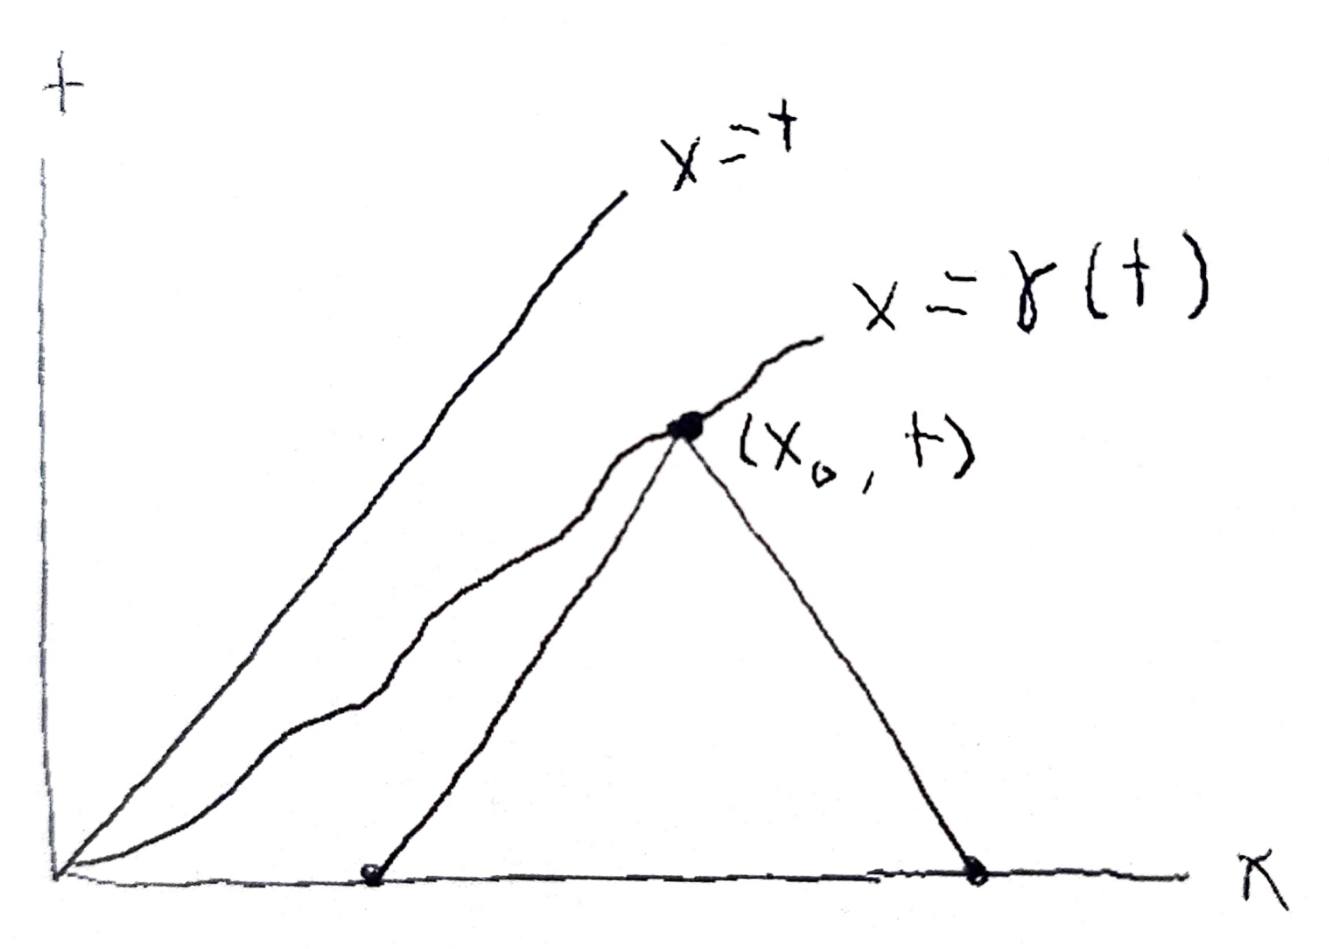
\includegraphics[width = 0.35\textwidth]{images/a.png}
		\end{figure}
		From the figure, we can see that when $ x_0 > \gamma(t_0) $, $ u(x_0, t_0) $ will be given by d'Alembert's solution. Furthermore, if we go up to the boundary (i.e. $ x_0 = \gamma(t_0) $), then $ u(x_0, t_0) $ can also be given by d'Alembert be both left and right going characteristics touch at $ (x_0, t_0) $. But, we must also have $ u(x_0, t_0) = u(\gamma(t0) = h(t) $ which will almost be equal to d'Alembert's solution. So we don't necessarily have existence along $ x = \gamma(t) $ and so our IBVP is not well-posed for $ \dot(\gamma) > 0 $.
		
		\item Is the IBVP with $ \dot{\gamma}(t) < -1 $ for some $ t > 0 $ well-posed?
		
		Below is a rough sketch of our solution space
		\begin{figure}[h!]
			\centering
			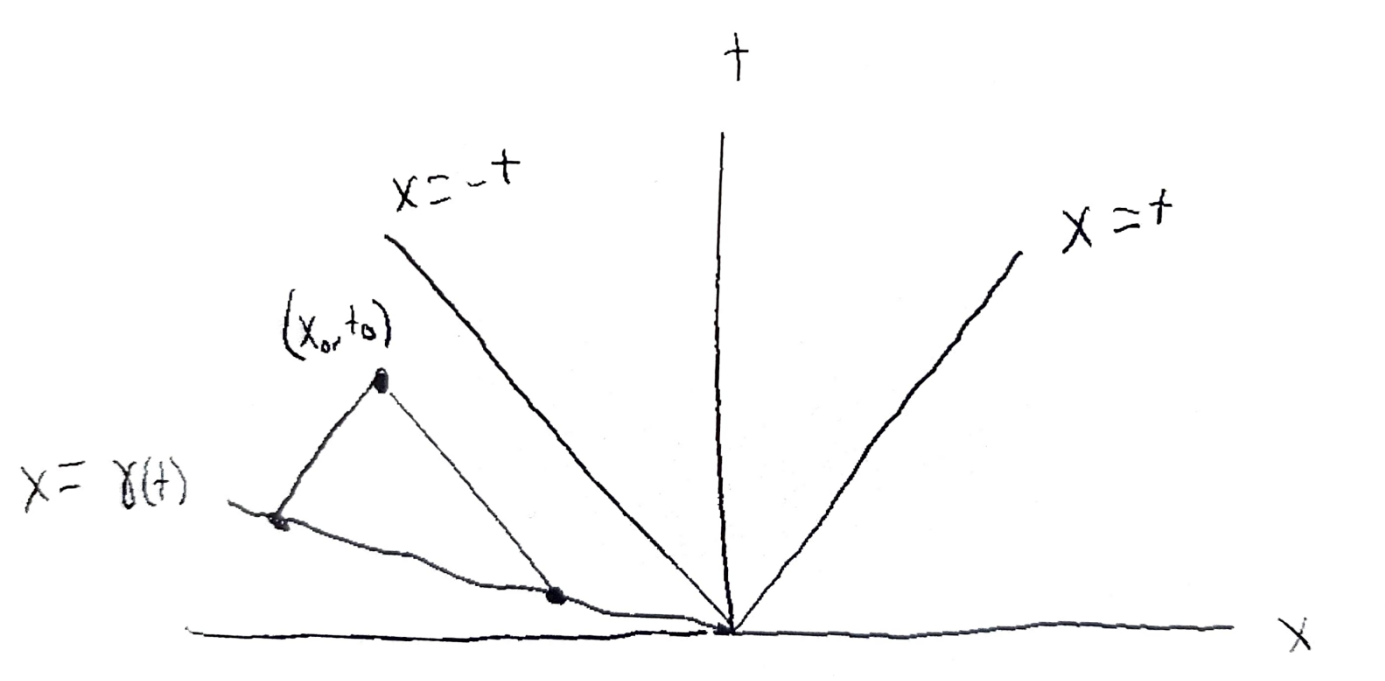
\includegraphics[width = 0.45\textwidth]{images/b.png}
		\end{figure}
		From the sketch, we can see that when $ \gamma(t_0) < x_0 < t_0 $, both left and right moving characteristics originate from the line $ x = \gamma(t) $ for $ t > 0 $. Furthermore, we know the general solution has the for $ u(x_0, t_0) = F(x_0 - t_0) + G(x_0 + t_0) $ which means that we have two unknowns to find to obtain our explicit solution. But, because the solution is only given information from $ x = \gamma(t) $, we only have the initial condition involving $ h(t) $. We don't have derivative information or other constraints for $ u(x_0, t_0) $ when $ \gamma(t_0) < x_0 < t_0 $ and so we can not uniquely determine $ u $ in this region. Therefore, the IBVP is ill-posed when $ \dot{\gamma} < -1 $.
		
		\item Solve the IBVP.
		
		First, let's assume $ \dot{\gamma(t)} \in (-1, 1) $ for all $ t > 0 $ so that we have a well-posed problem. Then, if $ x_0 > t_0 $, $ u(x_0,t_0) $ only has a domain of dependence involving $ f(x) $ and $ g(x) $. Therefore, when $ x_0 > t_0 $, $ u $ is given by d'Alembert's solution
		\[
			u(x_0, t_0) = \frac{1}{2}(f(x_0 - t_0) + f(x_0 - t_0)) + \frac{1}{2}\int_{x_0 - t_0}^{x_0 + t_0} g(y) \dd y.
		\]
		Now, if $ \gamma(t_0) < x_0 < t $, our solution is given by the domain of dependence $ D $ shown in the figure above.
		\begin{figure}[ht!]
			\centering
			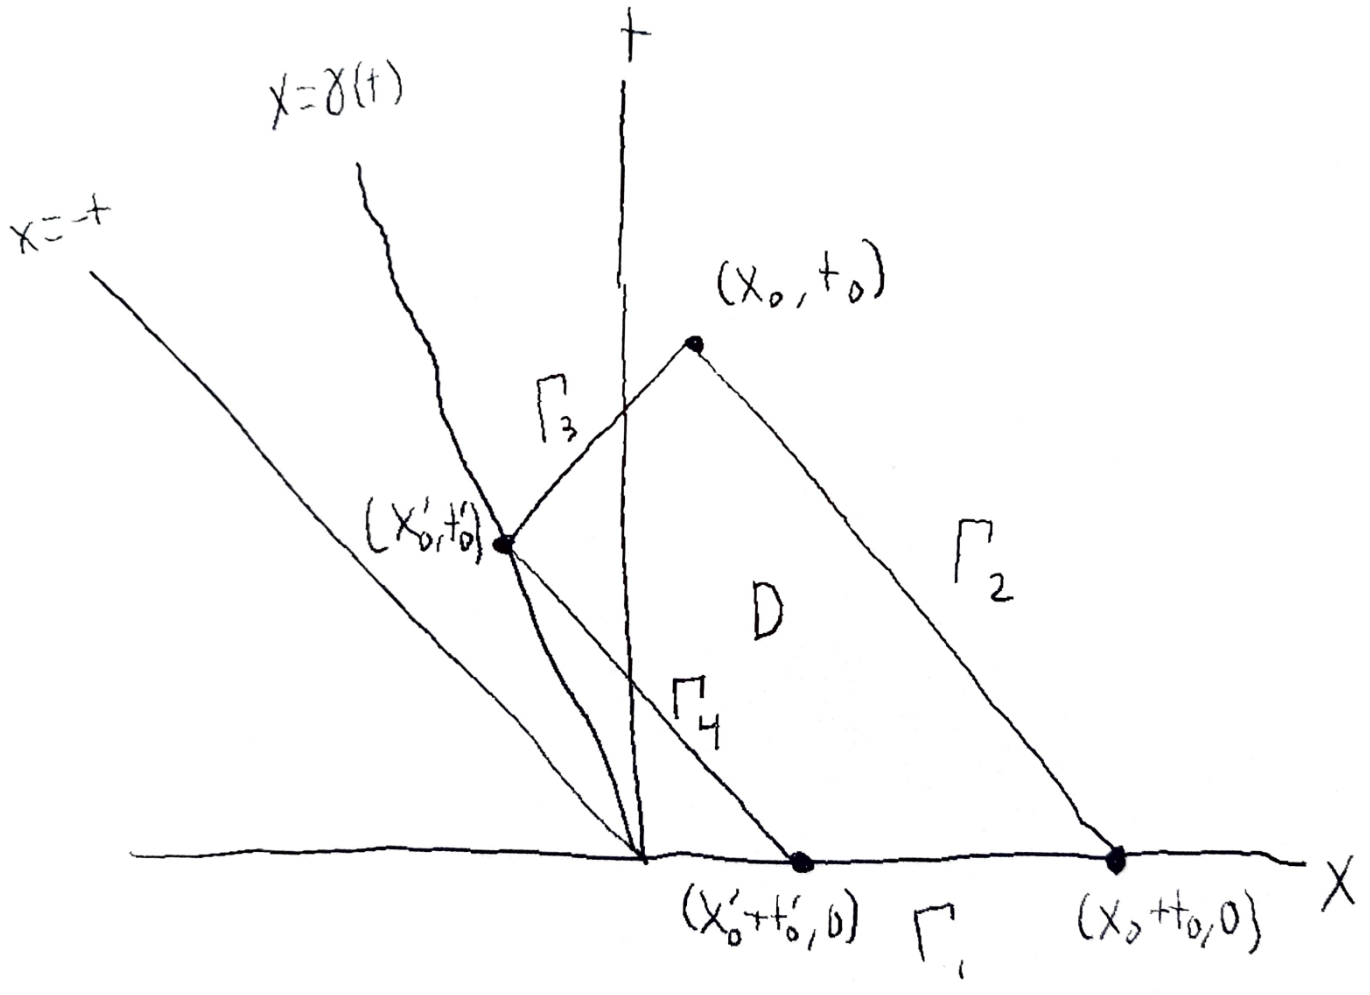
\includegraphics[width = 0.45\textwidth]{images/c.png}
		\end{figure}
		We can rewrite the PDE in terms of a vector quantity as
		\[
			u_{tt} - u_{xx} = \nabla \cdot \pmat{-u_x \\ u_t} = 0
		\]
		which implies
		\[
			\int_D \nabla \cdot \pmat{-u_x \\ u_t} \dd A = 0.
		\]
		Then, by the divergence theorem, we have
		\[
			\int_\Gamma \pmat{-u_x \\ u_t} \dd \textbf{S} = 0.
		\]
		From the figure, we can break this line integral into integrating counter-clockwise over $ \Gamma_1, \Gamma_2, \Gamma_3, $ and $ \Gamma_4 $. Before we continue, let $ (x_0',t_0') $ be the point that satisfies both
		\begin{align*}
			t_0' - t_0 &= x_0' - x_0 \\
			\shortintertext{and}
			x_0' &= \gamma(t_0').
		\end{align*}
		 Then, our parameterizations of the different lines can be as follows
		\begin{align*}
			\Gamma_1: & (x(s), t(s)) = (s, 0) \\
			\Gamma_2: & (x(s), t(s)) = (s, -(s - x_0) + t_0) \\
			\Gamma_3: & (x(s), t(s)) = (s, s - x_0' + t_0') \\
			\Gamma_4: & (x(s), t(s)) = (s, -(s - x_0') + t_0')
		\end{align*}
		Now let's break up our integral into manageable chunks
		\[
			\int_{\Gamma} \pmat{-u_x \\ u_t} \dd \textbf{S} = \int_{\Gamma_1} \pmat{-u_x \\ u_t} \dd \textbf{S} + 
			\int_{\Gamma_2} \pmat{-u_x \\ u_t} \dd \textbf{S} + 
			\int_{\Gamma_3} \pmat{-u_x \\ u_t} \dd \textbf{S} + 
			\int_{\Gamma_4} \pmat{-u_x \\ u_t} \dd \textbf{S} = 0.
		\]
		So for $\Gamma_1$, we have
		\[
			\dd \textbf{S} = \pmat{0 \\ -1} \dd s \text{ with } x_0' + t_0' \leq s \leq x_0 + t_0
		\]
		which yields
		\begin{align*}
			\int_{\Gamma_1} \pmat{-u_x \\ u_t} \dd \textbf{S} &= \int_{x_0' + t_0'}^{x_0 + t_0} \pmat{-u_x \\ u_t}\cdot \pmat{0 \\ -1} \dd s \\
			&= \int_{x_0' + t_0'}^{x_0 + t_0} -u_t \dd s \\
			&= -\int_{x_0' + t_0'}^{x_0 + t_0} g(s) \dd s.
		\end{align*}
		Now, for $ \Gamma_2 $, we have 
		\[
			\frac{\dd u}{\dd s} = -u_x + u_t, \quad \dd \textbf{S} = \pmat{1 \\ 1} \dd s, \text{ with } x_0 \leq s \leq x_0 + t_0
		\]
		which yields
		\begin{align*}
			\int_{\Gamma_2} \pmat{-u_x \\ u_t} \dd \textbf{S} &= \int_{x_0 + t_0}^{x_0} \pmat{-u_x \\ u_t} \cdot \pmat{1 \\ 1} \dd s \\
			&= \int_{x_0 + t_0}^{x_0} -u_x + u_t \dd s \\
			&= \int_{x_0 + t_0}^{x_0} \frac{\dd u}{\dd s} \dd s \\
			&= u(x_0, t_0) - u(x_0 + t_0, 0) \\
			&= u(x_0, t_0) - f(x_0 + t_0).
		\end{align*}
		Next, for $ \Gamma_3 $, we have
		\[
			\frac{\dd u}{\dd s} = -u_x - u_t, \quad \dd \textbf{S} = \pmat{-1 \\ 1} \dd s, \text{ with } x_0' \leq s \leq x_0
		\]
		which yields
		\begin{align*}
			\int_{\Gamma_3} \pmat{-u_x \\ u_t} \dd \textbf{S} &= \int_{x_0}^{x_0'} \pmat{-u_x \\ u_t} \cdot \pmat{-1 \\ 1} \dd s \\
			&= \int_{x_0}^{x_0'} u_x + u_t \dd s \\
			&= -\int_{x_0}^{x_0'} \frac{\dd u}{\dd s} \dd s \\
			&= u(x_0, t_0) - u(x_0', t_0') \\
			&= u(x_0, t_0) - h(t_0').
		\end{align*}
		Finally, for $ \Gamma_4 $, we have
		\[
		\frac{\dd u}{\dd s} = u_x - u_t, \quad \dd \textbf{S} = \pmat{-1 \\ -1} \dd s, \text{ with } x_0' \leq s \leq x_0' + t_0'
		\]
		which yields
		\begin{align*}
			\int_{\Gamma_4} \pmat{-u_x \\ u_t} \dd \textbf{S} &= \int_{x_0'}^{x_0' + t_0'} \pmat{-u_x \\ u_t} \cdot \pmat{-1 \\ -1} \dd s \\
			&= \int_{x_0'}^{x_0' + t_0'} u_x - u_t \dd s \\
			&= \int_{x_0'}^{x_0' + t_0'} \frac{\dd u}{\dd s} \dd s \\
			&= u(x_0' + t_0', 0) - u(x_0', t_0') \\
			&= f(x_0' + t_0') - h(t_0').
		\end{align*}
		Putting everything together, we have
		\[
			\int_\Gamma \pmat{-u_x \\ u_t} \dd \textbf{S} = -\int_{x_0' + t_0'}^{x_0 + t_0} g(s) \dd s + u(x_0, t_0) - f(x_0 + t_0) + u(x_0, t_0) - h(t_0') + f(x_0' + t_0') - h(t_0') = 0
		\]
		 which implies 
		 \[
		 	u(x_0, t_0) = \frac{1}{2}(f(x_0 + t_0) - f(x_0' + t_0')) + h(t_0') + \frac{1}{2} \int_{x_0' + t_0'}^{x_0 + t_0} g(s) \dd s
		 \]
		 for $ \gamma(t_0) < x_0 < t $.
		 
		 To briefly check our solution, let's assume $ \gamma(t) = 0 $. Then $ (x_0', t_0') = (0, t_0 - x_0) $ and so our solution is given by
		 \[
		 	u(x_0, t_0) = \begin{cases}
		 		\frac{1}{2}(f(x_0 - t_0) + f(x_0 + t_0)) + \frac{1}{2} \int_{x_0 - t_0}^{x_0 + t_0} g(s) \dd s, & x_0 > t_0 \\
		 		\frac{1}{2}(f(x_0 + t_0) - f(t_0 - x_0)) + h(t_0 - x_0) + \frac{1}{2}\int_{t_0 - x_0}^{x_0 + t_0}g(s) \dd s, & 0 < x < t
		 	\end{cases}.
		 \]
		 Which is exactly what we saw in class and in the book! We can see that the odd extension of $ f $ negatively interferes with the original left moving wave as expected.
	\end{enumerate}
	
	\newpage
	\item Consider the Euler-Poisson-Darboux (EPD) equation
	\[
		z_{\xi \eta} + \frac{N}{\xi + \eta} (z_\xi + z_\eta) = 0, z = z(\xi, \eta)
	\]	
	for $ N $ a natural number.
	\begin{enumerate}[label = (\alph*)]
		\item Verify that
		\[
			z(\xi, \eta) = k + \frac{\partial^{N - 1}}{\partial \xi^{N - 1}} \left(\frac{f(\xi)}{(\xi + \eta)^N}\right) + \frac{\partial^{N - 1}}{\partial \eta^{N - 1}} \left(\frac{g(\eta)}{(\xi + \eta)^N}\right)
		\]
		for $ k \in \reals $ and $ f,g $ sufficiently smooth function, is the general purpose solution to the EPD equation. \textit{Hint:} We have the identity
		\[
			\frac{\partial^{N}}{\partial \xi^{N}} \left(\frac{f(\xi)}{(\xi + \eta)^N}\right) = (\xi + \eta)\frac{\partial^{N}}{\partial \xi^{N}} \left(\frac{f(\xi)}{(\xi + \eta)^{N + 1}}\right) + N\frac{\partial^{N - 1}}{\partial \xi^{N - 1}} \left(\frac{f(\xi)}{(\xi + \eta)^{N + 1}}\right).
		\]
		
		To verify the solution, let's compute our need partials:
		\begin{align*}
			z_\xi &= \frac{\partial^{N}}{\partial \xi^{N}} \left(\frac{f(\xi)}{(\xi + \eta)^N}\right) + \frac{\partial^{N - 1}}{\partial \eta^{N - 1}}\frac{\partial}{\partial \xi} \left(\frac{g(\eta)}{(\xi + \eta)^N}\right) \\
			&= (\xi + \eta)\frac{\partial^{N}}{\partial \xi^{N}} \left(\frac{f(\xi)}{(\xi + \eta)^{N + 1}}\right) + N\frac{\partial^{N - 1}}{\partial \xi^{N - 1}} \left(\frac{f(\xi)}{(\xi + \eta)^{N + 1}}\right) - N \frac{\partial^{N - 1}}{\partial \eta^{N - 1}} \left(\frac{g(\eta)}{(\xi + \eta)^{N + 1}}\right) \\
			z_\eta &= \frac{\partial^{N - 1}}{\partial \xi^{N - 1}} \frac{\partial}{\partial \eta}\left(\frac{f(\xi)}{(\xi + \eta)^N}\right) + \frac{\partial^{N}}{\partial \eta^{N}} \left(\frac{g(\eta)}{(\xi + \eta)^N}\right) \\
			&= -N\frac{\partial^{N - 1}}{\partial \xi^{N - 1}} \left(\frac{f(\xi)}{(\xi + \eta)^{N + 1}}\right) + (\xi + \eta)\frac{\partial^{N}}{\partial \eta^{N}} \left(\frac{g(\eta)}{(\xi + \eta)^{N + 1}}\right) + N\frac{\partial^{N - 1}}{\partial \eta^{N - 1}} \left(\frac{g(\eta)}{(\xi + \eta)^{N + 1}}\right) \\
			z_{\xi \eta} &= \frac{\partial^{N}}{\partial \xi^{N}} \frac{\partial}{\partial \eta} \left(\frac{f(\xi)}{(\xi + \eta)^N}\right) + \frac{\partial^{N}}{\partial \eta^{N}} \frac{\partial}{\partial \xi} \left(\frac{g(\eta)}{(\xi + \eta)^N}\right) \\
			&=-N\frac{\partial^{N}}{\partial \xi^{N}} \left(\frac{f(\xi)}{(\xi + \eta)^{N + 1}}\right) - N\frac{\partial^{N}}{\partial \eta^{N}} \left(\frac{g(\eta)}{(\xi + \eta)^{N + 1}}\right).
		\end{align*}
		Then with two cancellations, we have
		\begin{align*}
			\frac{N}{\xi + \eta} (z_\xi + z_\eta) &= \frac{N}{\xi + \eta} \left((\xi + \eta)\frac{\partial^{N}}{\partial \xi^{N}} \left(\frac{f(\xi)}{(\xi + \eta)^{N + 1}}\right) + (\xi + \eta)\frac{\partial^{N}}{\partial \eta^{N}} \left(\frac{g(\eta)}{(\xi + \eta)^{N + 1}}\right)\right) \\
			&= N\frac{\partial^{N}}{\partial \xi^{N}} \left(\frac{f(\xi)}{(\xi + \eta)^{N + 1}}\right) + N\frac{\partial^{N}}{\partial \eta^{N}} \left(\frac{g(\eta)}{(\xi + \eta)^{N + 1}}\right).
		\end{align*}
		From here, it is easy to see that the rest cancels to get
		\[
			z_{\xi \eta} + \frac{N}{\xi + \eta} (z_\xi + z_\eta) = 0.
		\]
		Therefore, $ z(\xi, \eta) $ is a solution to the EPD equation.
		
		\item Show that if $ z $ satisfies the EPD equation, then $ u(r, t) = z(r + t, r - t) $ satisfies the wave-type equation
		\[
			u_{tt} - u_{rr} - \frac{2N}{r} u_r = 0.
		\]
		
		With $ u(r, t) = z(r + t, r - t) $, we must have $ \xi = r + t $ and $ \eta = r - t $ which implies
		\[
			\xi + \eta = 2r \implies r = \frac{1}{2}(\xi + \eta).
		\]
		Now, let's compute some needed partials
		\begin{align*}
			u_t &= z_\xi - z_\eta \\
			u_{tt} &= z_{\xi\xi} - 2 z_{\xi \eta} + z_{\eta \eta} \\
			u_r &= z_\xi + z_\eta \\
			u_{rr} &= z_{\xi\xi} + 2 z_{\xi \eta} + z_{\eta \eta}.
		\end{align*}
		Next, using these partials, we have
		\begin{align*}
			u_{tt} - u_{rr} - \frac{2N}{r} &= z_{\xi\xi} - 2 z_{\xi \eta} + z_{\eta \eta} - z_{\xi\xi} - 2 z_{\xi \eta} - z_{\eta \eta} - \frac{2N}{r} (z_\xi + z_\eta) \\
			&= -4 z_{\xi \eta} - \frac{2N}{r}(z_\xi + z_\eta) \\
			&= -4 z_{\xi \eta} - \frac{2N}{\frac{1}{2}(\xi + \eta)}(z_\xi + z_\eta) \\
			&= -4 \left(z_{\xi \eta} - \frac{N}{\xi + \eta}(z_\xi + z_\eta)\right) \\
			&= -4 (0) \\
			&= 0.
		\end{align*}
		Therefore, $ u(r,t) = z(r+t, r-t) $ is a solution to the wave-type equation.
		
		\item The wave equation in $ n $ dimensions is
		\[
			u_{tt} - \Delta u = 0
		\]
		where $ x \in \reals^n $. Prove that radial solutions in the form of $ u(x, t) = v(\norm{x}, t) $, depending only on $ r = \norm{x} $, satisfy
		\[
			v_{tt} - v_{rr} - \frac{n - 1}{r}v_r = 0
		\]
		implying that, when $ N = \frac{1}{2}(n - 1) $, $ n $ is an odd number, the EPD equation is equivalent to the radial wave equation.
		
		Suppose $ u(x, t) = v(\norm{x}, t) $. Then the second time derivative is given by
		\[
			u_{tt} = v_{tt}(\norm{x}, t).
		\]
		Furthermore, the Laplacian can be computed as
		\begin{align*}
			\Delta u = \Delta v &= \sum_{i = 1}^{n} \partial_{x_i x_i} v(\norm{x}, t) \\
			&= \sum_{i=1}^{n} \partial_{x_i} \left(v_r \frac{x_i}{\norm{x}}\right) \\
			&= \sum_{i = 1}^{n} \left(v_{rr} \frac{x_i^2}{\norm{x}^2} + v_r \frac{\norm{x} - \frac{x_i^2}{\norm{x}}}{\norm{x}^2}\right) \\
			&= v_{rr} \frac{1}{\norm{x}^2} \underbrace{\sum_{i = 1}^{n} x_i^2}_{\norm{x}^2} + \frac{v_r}{\norm{x}} \left(\underbrace{\sum_{i = 1}^{n} (1)}_n - \frac{1}{\norm{x}^2} \underbrace{\sum_{i = 1}^{n}x_i^2}_{\norm{x}^2}\right) \\
			&= v_{rr} + \frac{v_r}{\norm{x}}(n - 1) \\
			&= v_{rr} + \frac{n - 1}{r}v_r.
		\end{align*}
		Then, putting everything together, we have
		\[
			0 = u_{tt} - \Delta u = v_{tt} - v_{rr} - \frac{n - 1}{r}v_r.
		\]
		Therefore $ v $ satisfies the radial wave equation.
		
		\item What is the general solution to the radial wave equation for an odd number of dimensions?
		
		Let $ x \in \reals^n $ with $ n $ odd. Then by part (c) if $ N = \frac{1}{2} (n - 1) $, we have the solution to the radial wave equation in odd dimensions
		\[
			v_{tt} - v_{rr} - \frac{n - 1}{r} v_r = 0
		\]
		which is given by
		\[
			u(x, t) = v(\norm{x}, t) = v(r, t) = z(r + t, r - t)
		\]
		where from part (b) and (a),
		\[
			u(x,t) = z(r + t, r - t) = k + \left.\frac{\partial^{N - 1}}{\partial \xi^{N - 1}} \left(\frac{f(\xi)}{(\xi + \eta)^N}\right)\right|_{\xi = r + t, \eta = r - t} + \left.\frac{\partial^{N - 1}}{\partial \eta^{N - 1}} \left(\frac{g(\eta)}{(\xi + \eta)^N}\right)\right|_{\xi = r + t, \eta = r - t}
		\]
		with $ r = \norm{x} $.
	\end{enumerate}
\end{enumerate}
\end{document}
